%This is a Latex file.
\documentclass[12pt]{article}
\usepackage{latexsym,fancyhdr,amsmath,amsfonts,amsthm,dsfont}
\usepackage{amssymb}

\usepackage{graphicx} 

% margins are relative to the default of 1 in
%\topmargin       -0.2 in

\topmargin        -0.2 in
\textheight       8.4 in
\oddsidemargin    0 in     % this is for pages 1, 3, 5, ...
\evensidemargin   0 in     % and this for 2, 4, 6, ...
\textwidth        6.5 in
%\headheight       15 in     % we won't have a running head, nor
\headsep          .35 in     % any extra space between head and text

%\parindent 0pt

\pagestyle{fancy} \lhead{\sf MTH 317} \chead{\sf Homework 4}
\rhead{\sf Rayana Gottschall} \lfoot{} \cfoot{} \rfoot{}

\newcommand{\C}{\mathds{C}}
\newcommand{\I}{\mathds{I}}
\newcommand{\N}{\mathds{N}}
\newcommand{\Q}{\mathds{Q}}
\newcommand{\R}{\mathds{R}}
\newcommand{\Z}{\mathds{Z}}

\begin{document}
\begin{enumerate}
\item[2.38] For the adjacency matrix A, determine $A^2$ and $A^3$.
\newline
$A^2$ =
\[
\begin{bmatrix}
2 & 1 & 1 & 1 & 0 \\
1 & 2 & 1 & 1 & 0  \\
1 & 1 & 3 & 0 & 1 \\
1 & 1 & 0 & 2 & 0  \\ 
0 & 0 & 1 & 0 & 1
\end{bmatrix}
\]

$A^3$ =
\[
\begin{bmatrix}
2 & 3 & 4 & 1 & 1 \\
3 & 2 & 4 & 1 & 1  \\
4 & 4 & 2 & 4 & 0 \\
1 & 1 & 4 & 0 & 2  \\ 
1 & 1 & 0 & 2 & 0
\end{bmatrix}
\]
 
\item[2.41] 
\item[] a) Compute $BB^t$
\item[] $BB^t$ =
\[
\begin{bmatrix}
3 & 1 & 1 & 1 & 0 \\
1 & 2 & 0 & 1 & 0  \\
1 & 0 & 2 & 1 & 0 \\
1 & 1 & 1 & 4 & 1  \\ 
0 & 0 & 0 & 1 & 1
\end{bmatrix}
\]
\item[] b) What does the ($i, j$) entry of $BB^t$ represent?
\newline
The $i$ is the vertex and the $j$ is the edge. 0 means there is no connection, 1 means there is a connection. 
And the diagonal entries represent the degrees for each vertex.

\item[3.2] Give an example of 3 graphs of the same size, order, and degree sequence that are not isomorphic to one another.
\newline
\begin{center}
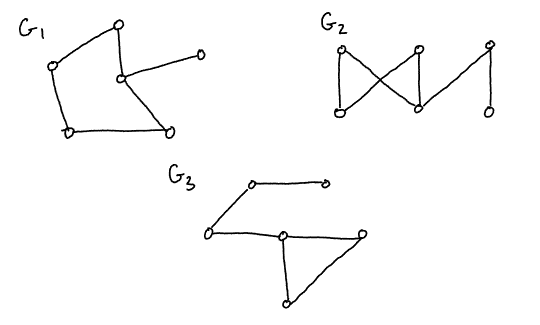
\includegraphics{graph.png}
\end{center}
Here each graph has order 6, size 6, and degree sequence (3, 2, 2, 2, 2, 1) but they are not isomorphic to one another.

\item[4.2] Prove every connected graph with even degrees contains no bridges.
\begin{proof}
    Let G be a connected graph with all vertices of even degree. 
    Since all degrees are even, G is not a tree. Because G cannot contain a leaf (vertex
    of degree 1). Since G is connected, not a tree, and only has even degrees, 
    every edge of G must lie on a cycle. But by Theorem 4.1, no edge of a cycle is a bridge.
    So G cannot contain a bridge.
\end{proof}

 
\item[4.4] Let G be a connected graph and let $e_1$ and $e_2$ be two edges of G.
Prove that G -$e_1$ -$e_2$ has three components if and only if $e_1$ and $e_2$ are bridges.
\begin{proof}
     ($\Rightarrow$) Assume G -$e_1$ -$e_2$ has three components and $e_1$ and $e_2$
        have distinct vertices.
        Since G is connected, removing $e_1$ and $e_2$ must have increased the 
        number of components from 1 to 3. So,  $e_1$ and $e_2$ are bridges.
    \newline
    ($\Leftarrow$) Assume $e_1$ and $e_2$ are bridges with distinct vertices.
        Since G is connected and has 2 bridges, removing $e_1$ and $e_2$ must 
        increase the number of components from 1 to 3. So, G -$e_1$ -$e_2$ has three components.
\end{proof}

\end{enumerate}
\end{document}
